\documentclass[tikz,border=5pt]{standalone}
\usepackage{amsmath}
\usetikzlibrary{positioning,arrows.meta}

\begin{document}
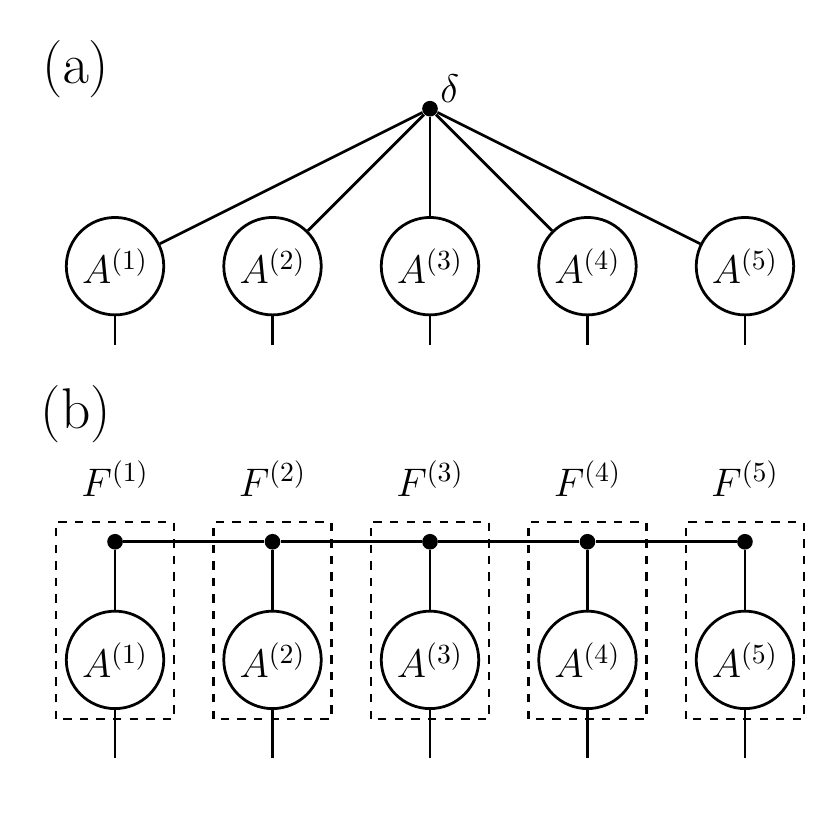
\begin{tikzpicture}[
  node/.style={circle,draw,inner sep=3pt,line width=1pt},
  level distance=1.2cm,
  sibling distance=1.6cm
]

\Large

% (a)
\node at (-4.5,1.5) {\huge{(a)}};
\node at (0.25,1.25) {$\delta$};
\node[fill, circle, inner sep=2pt] (rootB) at (0,1) {};
\node[node] (A1) at (-4,-1) {$A^{(1)}$};
\node[node] (A2) at (-2,-1) {$A^{(2)}$};
\node[node] (A3) at (0,-1)  {$A^{(3)}$};
\node[node] (A4) at (2,-1)  {$A^{(4)}$};
\node[node] (A5) at (4,-1)  {$A^{(5)}$};

\foreach \i in {1,2,3,4,5}
  \draw[line width=1pt] (rootB) -- node[]{} (A\i);
%\node[] at (0.25,-0.5) {$R$};

\foreach \i in {1,2,3,4,5}
  \draw[line width=1pt] (A\i) -- ++(0,-1) node[below]{};
%  \draw[line width=1pt] (A\i) -- ++(0,-1) node[below]{$d_{\i}$};

% (b)
\node at (-4.5,-2.875) {\huge{(b)}};
\node[fill, circle, inner sep=2pt] (rootD1) at (-4,-4.5) {};
\node[fill, circle, inner sep=2pt] (rootD2) at (-2,-4.5) {};
\node[fill, circle, inner sep=2pt] (rootD3) at (0,-4.5) {};
\node[fill, circle, inner sep=2pt] (rootD4) at (2,-4.5) {};
\node[fill, circle, inner sep=2pt] (rootD5) at (4,-4.5) {};
\node[node] (A1) at (-4,-6) {$A^{(1)}$};
\node[node] (A2) at (-2,-6) {$A^{(2)}$};
\node[node] (A3) at (0,-6) {$A^{(3)}$};
\node[node] (A4) at (2,-6) {$A^{(4)}$};
\node[node] (A5) at (4,-6) {$A^{(5)}$};

\foreach \i/\j in {1/2,2/3,3/4,4/5}
  \draw[line width=1pt] (rootD\i) -- node[above]{} (rootD\j);

\foreach \i in {1,2,3,4,5}
  \draw[line width=1pt] (A\i) -- node[above, yshift=25pt]{$F^{(\i)}$} (rootD\i);

\foreach \i in {1,2,3,4,5}
  \draw[line width=1pt] (A\i) -- ++(0,-1.25) node[below]{};

\foreach \i in {1,2,3,4,5}
  \draw[dashed, line width=1pt] (A\i) ++(-0.75,-0.75) rectangle ++(1.5,2.5);

\end{tikzpicture}
\end{document}

